\section{Method}

\begin{figure}[t]
\centering
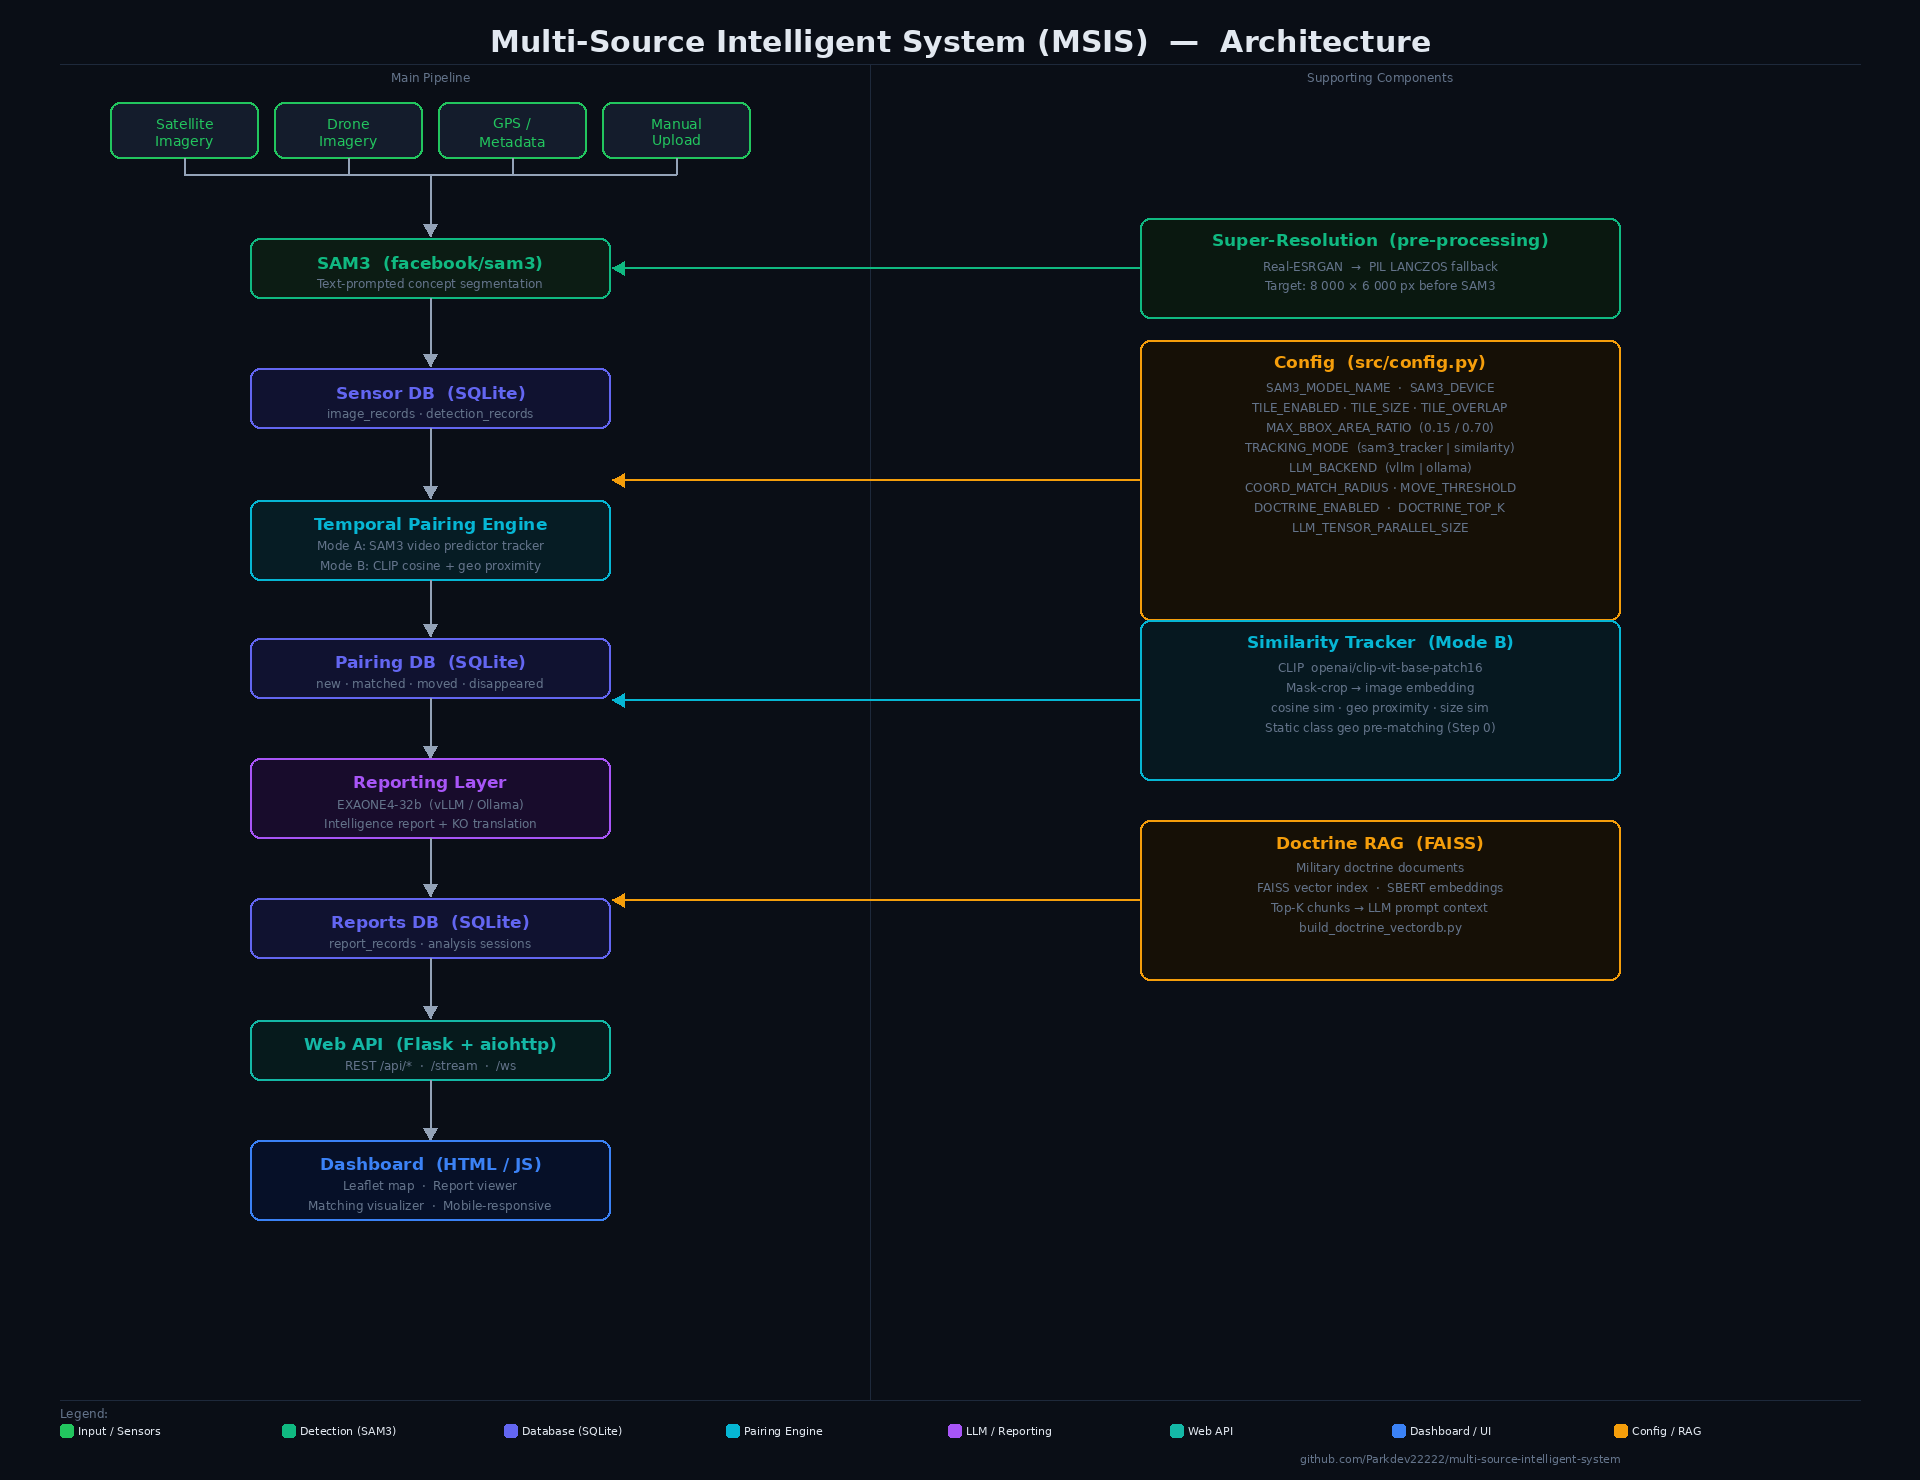
\includegraphics[width=\columnwidth]{../docs/architecture.png}
\caption{Pipeline. Two revisits are segmented independently; detections are
geo-referenced; the learned head matches instances across frames and verifies
the unmatched ones; survivors are written to a persistent spatio-temporal graph
that the report is generated from.}
\label{fig:architecture}
\end{figure}

\subsection{Pipeline}

Two co-registered revisits of a tile enter; a report leaves. An
open-vocabulary segmenter (\DetectorName) proposes object instances in each
frame independently, at three scales, with non-maximum suppression across
scales. Each detection is geo-referenced through an invertible
pixel-to-latitude/longitude transform, so every downstream stage reasons in
world coordinates rather than tile coordinates and observations of the same
place from different tiles or dates coincide.

The pairing head then decides, for candidate detection pairs across the two
frames, which are the same physical object, and for detections left unmatched,
which represent a genuine change. Surviving instances are written into a
persistent spatio-temporal knowledge graph keyed by location, so a
neighbourhood accumulates entity histories across revisits. The report is
generated from that structure rather than from the images.

\subsection{Learned Pairing}

Let $P$ and $C$ be the detections in the past and current frames. Candidate
pairs are formed within a geographic radius. For each candidate we compute
\NPairFeatures{} pair features: CLIP cosine between mask-cropped patches,
geodesic centre distance normalised by the match radius, IoU of the
geo-referenced boxes, log area ratio, aspect difference, both confidences,
class agreement, signed centre offsets, mutual-best-match indicators for CLIP
and geometry, normalised candidate ranks, and candidate densities on both
sides. The rank and density features matter more than they look: they let the
head condition on how contested a match is, which a pairwise similarity alone
cannot express.

For each detection we compute \NUnaryFeatures{} unary features: confidence,
log relative area, aspect, position in the tile, mask fill ratio (a proxy for
segmentation quality), the best geometric and CLIP agreement it finds in the
other frame, the number of overlapping detections there, distance to the tile
edge, and \NCrossFrameFeatures{} cross-frame features described below.

Three small multi-layer perceptrons share a class embedding
(Fig.~\ref{fig:architecture}): $\mathrm{match}$ scores a candidate pair,
$\mathrm{state}$ classifies a matched pair as stationary, moved or modified,
and $\mathrm{verify}$ scores whether an unmatched detection is a genuine change
instance. Each is two hidden layers of width 64 with layer normalisation, GELU
and dropout; features are standardised with statistics fitted on the training
split. The whole head is \HeadParams{} parameters.

Matching is a greedy assignment over $\mathrm{match}$ scores above a threshold;
we also report a variant using the Hungarian algorithm, which changes the
result by less than 0.1 F1. Unmatched detections are kept only if
$\mathrm{verify}$ exceeds its own threshold. Both thresholds are selected on
the validation split and never on test.

\textbf{Supervision is free.} Change-detection benchmarks publish binary change
masks. We convert a mask to instances by connected components, then label a
candidate pair positive when both detections fall outside the change region and
co-locate, and label an unmatched detection positive when it overlaps a
ground-truth change instance. No annotation beyond what the benchmark already
ships is required, which is what makes the head cheap to retrain for a new
sensor or region.

\subsection{Cross-Frame Co-located Evidence}

The dominant failure of any detect-then-pair design is asymmetric detector
recall. If the segmenter misses a building in the past frame and finds it in
the current one, pairing has nothing to pair against and the object is reported
as new construction. The evidence that it was already there is in the past
frame's pixels, not in its detections.

For every detection we therefore crop \emph{the same geographic footprint} from
both frames --- regardless of whether the detector fired in the other frame ---
and compute four quantities: CLIP cosine between the two crops, mean absolute
pixel difference, normalised cross-correlation, and signed edge-density change,
which rises sharply when a roof appears. These are handed to $\mathrm{verify}$
as features rather than compared against a fixed threshold, which is what the
production heuristic did.

Ablating this evidence requires \emph{retraining} without it, not zeroing it at
inference: after standardisation, zero is not a neutral input, so zeroing
measures a broken model rather than the feature's contribution. Retrained
without it, the head loses \EOneCrossFrameGain{} pixel F1 and
\EOneCrossFrameInstGain{} instance F1.

\subsection{Spatio-Temporal Knowledge Graph and Report Generation}

Verified instances are upserted into a graph keyed by geographic location:
entity nodes with observation histories, location nodes, and typed relations
between them. Community detection over the entity graph yields neighbourhood
summaries. On a revisit, an entity is matched to its own history by location,
so the graph accumulates rather than resets.

Report generation is conditioned on progressively more of this structure, which
gives the grounding ladder we ablate in Section~\ref{sec:experiments}:

\begin{itemize}
\item \texttt{template} --- deterministic prose from the change inventory, no
      language model. This is not a hallucination-free condition: it invents no
      sentences but states whatever the detector found, so every detection
      error becomes an unsupported claim. It fixes the error floor our own
      detector imposes.
\item \texttt{vlm\_direct} --- an external baseline: a vision--language model
      shown both images and none of our pipeline.
\item \texttt{llm\_raw} --- a language model over the unaggregated detection
      dump.
\item \texttt{llm\_struct} --- over the aggregated change inventory, isolating
      aggregation.
\item \texttt{llm\_flat\_rag} --- plus top-$k$ retrieved past observations,
      isolating whether \emph{any} history helps.
\item \texttt{llm\_graphrag} --- plus entity histories and community summaries.
\end{itemize}

\texttt{llm\_flat\_rag} is the condition that makes the comparison honest:
without it, a gain from graph grounding could be nothing more than ``retrieval
helps''.
